\documentclass{article}
\usepackage[utf8]{inputenc}
\usepackage{amsmath}
\usepackage{graphicx}
\usepackage{subcaption}

\DeclareMathOperator*{\minimize}{minimize}


\title{[FMAN45] - Assignment1}
\author{Filip Kalkan (fi1231ka-s) }
\date{April 2022}

\begin{document}

\maketitle

\section{Task 1}
We begin by differentiating the expression in
\begin{equation} \label{eq1}
    \displaystyle{\minimize_{\omega_i}}\text{ } \frac{1}{2} ||r_i - x_i \omega_i||_2^2 + \lambda|\omega_i|
\end{equation}
with respect to $\omega_i$.
\begin{equation} \label{eq2}
\begin{split}
\frac{d}{d\omega_i} \bigg(\frac{1}{2} ||r_i - x_i \omega_i||_2^2 + \lambda|\omega_i|\bigg) \\
 = \frac{1}{2} \bigg( 2(r_i - x_i\omega_i)(-x_i)\bigg) + \lambda \frac{\omega_i}{|\omega_i|} \\
 = (r_i-x_i\omega_i)(-x_i) + \lambda \frac{\omega_i}{|\omega_i|} \\
 = -x^T_i(r_i - x_i\omega_i) + \lambda \frac{\omega_i}{|\omega_i|}
\end{split}
\end{equation}

(\ref{eq1}) is equivalent to setting (\ref{eq2}) to 0.

\begin{equation} \label{eq3}
\begin{split}
0 = -x^T_i(r_i - x_i\hat{\omega_i}) + \lambda \frac{\hat{\omega_i}}{|\hat{\omega_i}|} \\
\Longleftrightarrow 0 = -x_i^Tr_i + x_i^Tx_i\hat{\omega_i} + \lambda \frac{\hat{\omega_i}}{|\hat{\omega_i}|} \\
\Longleftrightarrow x_i^Tr_i = x_i^Tx_i\hat{\omega_i} + \lambda \frac{\omega_i}{|\omega_i|} \\
\end{split}
\end{equation}
Now, we concider the equation by its absolute value.
\begin{equation}
|x_i^Tr_i| = |\hat{\omega_i}|\bigg|x_i^Tx_i + \lambda \frac{1}{|\hat{\omega_i}|}\bigg|
\end{equation}
$x_i^T x_i$ and $\lambda$ are positive, meaning that we can write the equation as
\begin{equation}
    |x_i^Tr_i| = |\hat{\omega_i}|\bigg(x_i^Tx_i + \lambda \frac{1}{|\hat{\omega_i}|}\bigg)
\end{equation}
Now, we can easily identify that the entire right hand side is positive. Thus, we can remove the absolute value of the left hand side.
\begin{equation}
    x_i^Tr_i = |\hat{\omega_i}|\bigg(x_i^T x_i + \lambda \frac{1}{|\hat{\omega_i}|}\bigg)
\end{equation}
\begin{equation} \label{eq7}
    \Longleftrightarrow |\hat{\omega_i}| = \frac{1}{x_i^T x_i}\bigg(|x_i^T r_i| - \lambda\bigg)
\end{equation}

In order to determine $sgn(\hat{\omega_i})$ we need to concider the last equation in (\ref{eq3}), where $x_i^T x_i$ and $\lambda$ are positive. Thus,
\begin{equation} \label{eq8}
    sgn(\hat{\omega_i}) = sgn(x_i^T r_i) = \frac{x_i^T r_i}{|x_i^T r_i|}
\end{equation}
Multiplying (\ref{eq7}) with (\ref{eq8}) yields
\begin{equation}
\begin{split}
    \hat{\omega_i} = sgn(\hat{\omega_i})|\hat{\omega_i}| = \frac{x_i^T r_i}{|x_i^T r_i|} \frac{1}{x_i^T x_i} \bigg(|x_i^T r_i| - \lambda \bigg) \\
    \Longleftrightarrow \hat{\omega_i} = \frac{x_i^T r_i}{x_i^T x_i |x_i^T r_i|} \bigg(||x_i^T r_i|| - \lambda \bigg) 
\end{split}
\end{equation}
which is what we wanted to show.

\section{Task 2}
We begin by rewriting
\begin{equation}
    \hat{\omega_i}^{(j)} = \frac{x_i^T r_i^{(j-1)}}{x_i^T x_i |x_i^T r_i^{(j-1)}|} \bigg(||x_i^T r_i^{(j-1)}|| - \lambda \bigg)
\end{equation}
by using that $x_i^T x_i = I$. This results in
\begin{equation} \label{eq11}
\begin{split}
    \hat{\omega_i}^{(j)} = \frac{x_i^T r_i^{(j-1)}}{|x_i^T r_i^{(j-1)}|} \bigg(||x_i^T r_i^{(j-1)}|| - \lambda \bigg) \\
    = x_i^T r_i^{(j-1)} - \lambda sgn(x_i^T r_i^{(j-1)})
\end{split}
\end{equation}
in order to further simplify the equation, we need to rewrite $x_i^T r_i^{(j-1)}$, where
\begin{equation}
    r_i^{(j-1)} = t - \sum_{l<i} x_l \hat{\omega_l}^{j} - \sum_{l<i} x_l \hat{\omega_l}^{j-1}
\end{equation}
as follows.
\begin{equation} \label{eq13}
\begin{split}
    x_i^T r_i^{(j-1)} = x_i^T ( t - \sum_{l<i} x_l \hat{\omega_l}^{j} - \sum_{l<i} x_l \hat{\omega_l}^{j-1}) \\
    = \bigg[ x_i^T x_l = 0 \text{ }\forall \text{ } l \ne i, \text{ } x_i^T x_i = 1\bigg] \\
    = x_i^T t
\end{split}
\end{equation}
Inserting (\ref{eq13}) into (\ref{eq11}) yields
\begin{equation} \label{eq14}
     \hat{\omega_i}^{(j)} = x_i^T t - \lambda sgn(x_i^T t)
\end{equation}
which shows that $\hat{\omega_i}^{(j)}$ does not depend on previous any previous estimations. Finally, we can show that the coordinate descent will converge after at most one full pass over the coordinates in $\omega$ as follows.
\begin{equation}
    \hat{\omega_i}^{(2)} - \hat{\omega_i}^{(1)} = (x_i^T t - \lambda sgn(x_i^T t)) - (x_i^T t - \lambda sgn(x_i^T t)) = 0
\end{equation}

These properties also apply for the case $|x_i^T r_i^{(j-1)}| < \lambda$ as $\hat{\omega_i}^{(j)} = 0$.

\section{Task 3}
Firstly, we note that 
\begin{equation}
    \hat{\omega_i}^{(j)} = x_i^T t - \lambda sgn(x_i^T t)
\end{equation}
as shown in (\ref{eq14}) and investigate what happes to $x_i^T t$ if we let $\sigma \to 0$.
\begin{equation}
    \lim\limits_{\sigma \to 0} x_i^T t = x_i^T X \omega^* = \omega^*
\end{equation}

The three cases we want to investigate are
\begin{equation} \label{case1}
    x_i^T r_i^{(j-1)} > \lambda ,
\end{equation}
\begin{equation} \label{case2}
    x_i^T r_i^{(j-1)} < -\lambda ,
\end{equation}
\begin{equation} \label{case3}
    |x_i^T r_i^{(j-1)}| \leq \lambda 
\end{equation}

In the case given by (\ref{case1}):
\begin{equation} \label{case1sol}
\begin{split}
    \lim\limits_{\sigma \to 0} E(\hat{\omega_i}^{(1)} - \omega_i^{*}) \\
    = \lim\limits_{\sigma \to 0} E(x_i^T t - \lambda sgn(x_i^T t) - \omega_i^{*}) \\
    = E(\hat{\omega_i}^{*} - sgn(\hat{\omega_i}^{*}) - \omega_i^{*}) \\
    = -\lambda E(sgn(\omega_i^{*})) = -\lambda
\end{split}
\end{equation}

In the case given by (\ref{case2}), we re-use the calculations from (\ref{case1sol}) but with a negative $\hat{\omega_i}^{*})$:
\begin{equation}
\begin{split}
    \lim\limits_{\sigma \to 0} E(\hat{\omega_i}^{(1)} - \omega_i^{*}) \\
    = E(\omega_i^{*} - sgn(\omega_i^{*}) - \omega_i^{*}) \\
    = -\lambda E(sgn(\omega_i^{*})) = \lambda
\end{split}
\end{equation}

In the final case given by (\ref{case3}), we note that $\hat{\omega_i}^{(1)} = 0$. Meaning that
\begin{equation}
\begin{split}
    \lim\limits_{\sigma \to 0} E(\hat{\omega_i}^{(1)} - \omega_i^{*}) \\
    = E(0 - \omega_i^{*}) \\
    = -\omega_i^{*}
\end{split}
\end{equation}

LASSO (or Least Absolute Shrinkage and Selection Operator) appears to be a great method for avoiding high variance in a model. However, as is shown in the results above, strong regularization (large $\lambda$) is likely to result in high bias and therefore an inaccurate model.

\section{Task 4}
In this task, a signal was reconstucted using LASSO regularization with 3 different $\lambda$. The original signal is a linear combination of two sinusoids with different frequencies. 

\begin{figure}[h]
\centering
   \begin{subfigure}{0.45\linewidth}
   \centering
   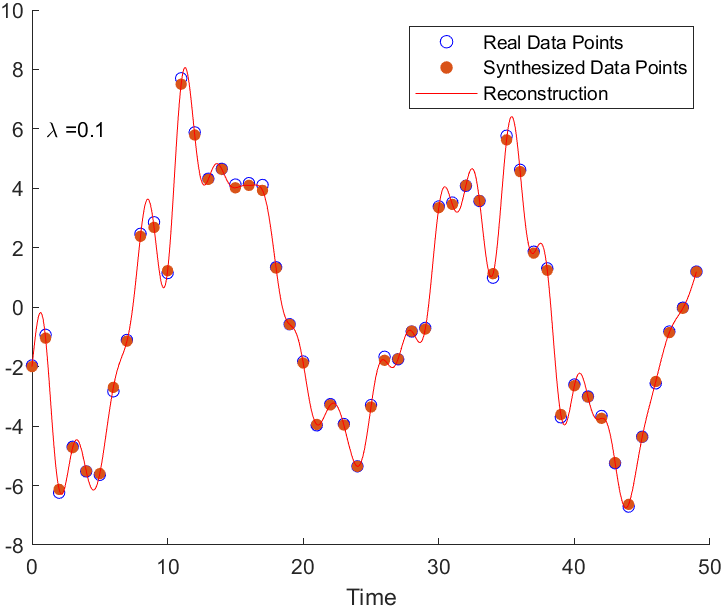
\includegraphics[width=\linewidth]{task41.png}
   \caption{}
   \label{fig:1} 
\end{subfigure}
\hfill
\begin{subfigure}{0.45\linewidth}
   \centering
   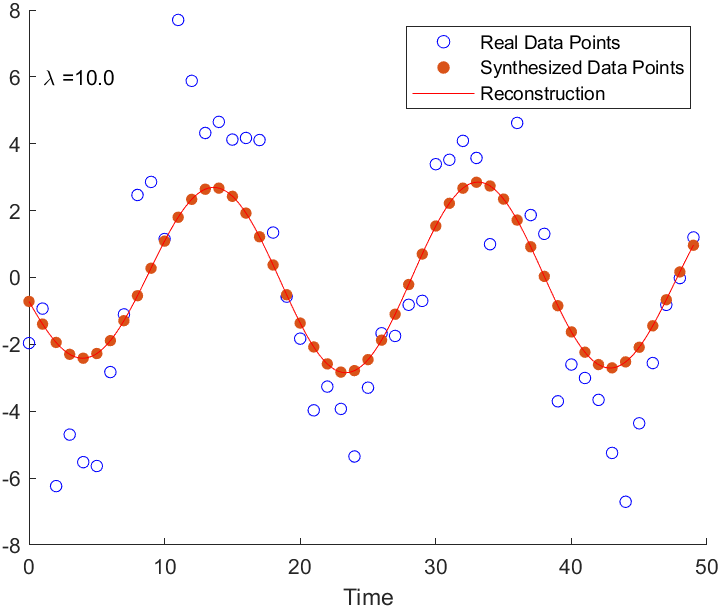
\includegraphics[width=\linewidth]{task42.png}
   \caption{}
   \label{fig:2}
\end{subfigure}
\\[\baselineskip]
\begin{subfigure}[h]{0.45\linewidth}
   \centering
   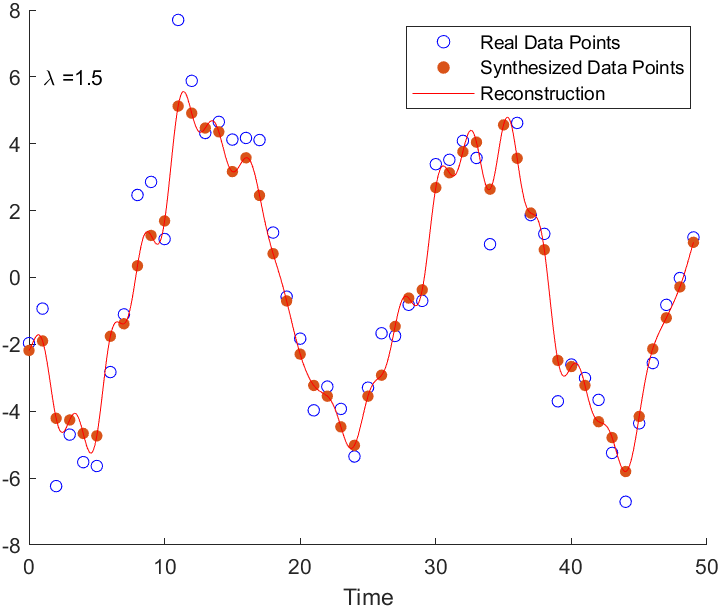
\includegraphics[width=\linewidth]{task43.png}
   \caption{}
   \label{fig:3}
\end{subfigure}
\centering
\caption{(a) Reconstruction plot using $\lambda = 0.1$. (b) Reconstruction plot using $\lambda = 10$. (c) Reconstruction plot using $\lambda = 1.5$.}
\end{figure}

In figure 1 (a) it is clearly visible that the model is overfitted as the real and synthesized data points overlap to a great extent. This means that the model is fitting to the noise in the signal as opposed to the actual original signal that we are trying to reproduce. This can be seen as the reconstruction line crosses all real data points.

Figure 1 (b) does not show any signs of overfitting, instead it appears that the model is underfitted. The reason being that the reconstruction line can be concidered far away from most real data points.

In contrast, figure 1 (c) shows a reasonable reconstruction of the signal. The line appears to be a linear combination of two sinusoids with different frequencies, while keeping a reasonable distance to the real data points. This indicates that the noise in the signal has been filtered out.


\begin{table}[h]
\centering
\resizebox{0.7\textwidth}{!}{%
\begin{tabular}{|l|l|l|}
\hline
$\lambda$    & Subfigure & Number of non-zero coordinates \\
\hline
0.1 & (a) & 253 \\
\hline
10 & (b) & 8 \\
\hline
1.5 & (c) & 61 \\
\hline
\end{tabular}%
}
\caption{Number of non-zero coordinates for each model presented in Figure 1.}
\centering
\end{table}

As indicated in table 1, there is an inversely proportional relation between $\lambda$ and the number of non-zero coordinates for the models presented. The table along with the figures also show that a reasonable reconstruction needs more non-zero coordinates than the actual explanatory variable consisting of 4 non-zero coordinates.

\section{Task 5}
In order to find the optimal $\lambda$ for reconstruction of the signal, the RMSE of the reconstruction using the validation data set was minimized. This was done using 10-fold cross validation with 100 different $\lambda$ values, where $\lambda \in [0.01, max(|X^T t|)]$. The results are shown in figure 2.
\begin{figure}[h]
\centering
   \begin{subfigure}{0.49\linewidth}
   \centering
   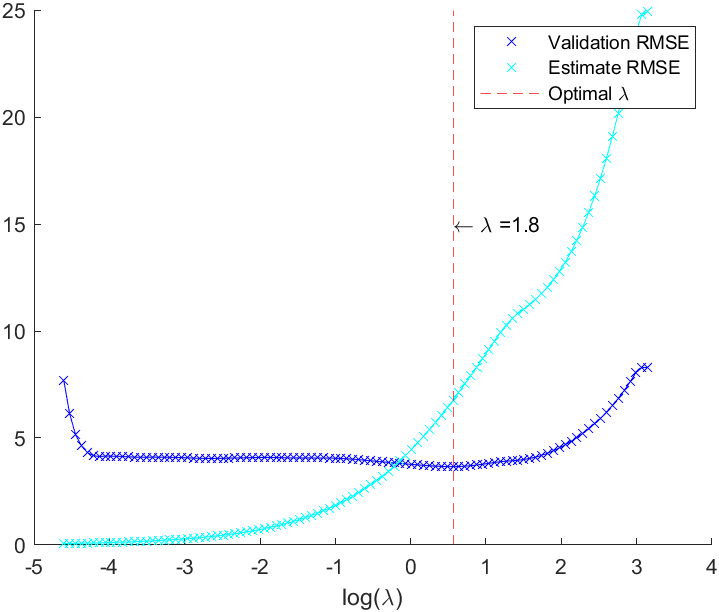
\includegraphics[width=\linewidth]{task51.png}
   \caption{}
   \label{fig:1} 
\end{subfigure}
\hfill
\begin{subfigure}{0.49\linewidth}
   \centering
   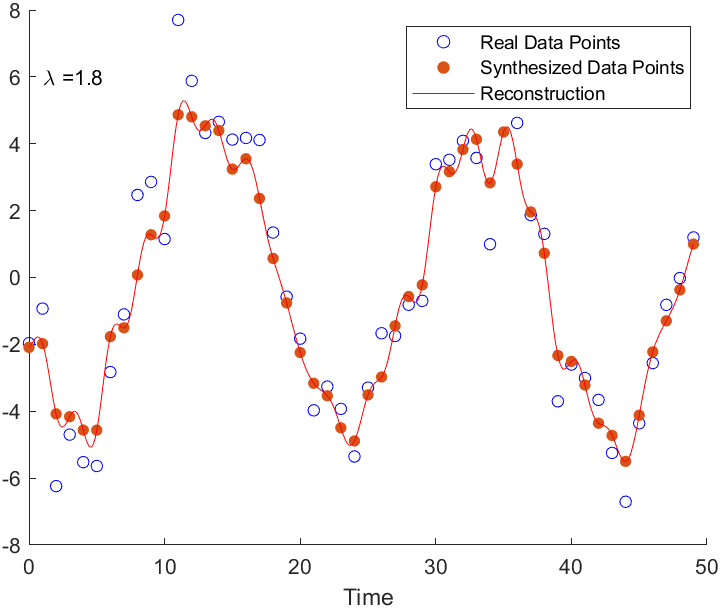
\includegraphics[width=\linewidth]{task52.png}
   \caption{}
   \label{fig:2}
\end{subfigure}
\caption{(a) Validation and estimation RMSE using 10-fold cross validation with 100 different $\lambda$. (b) Reconstruction using optimal $\lambda = 1.8$.}
\end{figure}
Using the optimal $\lambda = 1.8$ to construct our model, we get a fairly reasonable reconstruction of the signal (see Figure 2 (b)) as per the description of Figure 1 (c) under the section \textit{Task 4}.

\section{Task 6}
In order to find the optimal lambda across the frames of the audio exerpt, multiframe 3-fold cross validion was used. The RMSE for one $\lambda$ was calucated as the mean RMSE for that lambda across frames. The optimal $\lambda$ was obtained by identifying the $\lambda$ corresponding to the smallest validation RMSE.

In this task, $\lambda \in [0.00001, max(|X^T t_i|) \forall i]$ where $i$ is the frame index.

\begin{figure}[h]
    \centering
    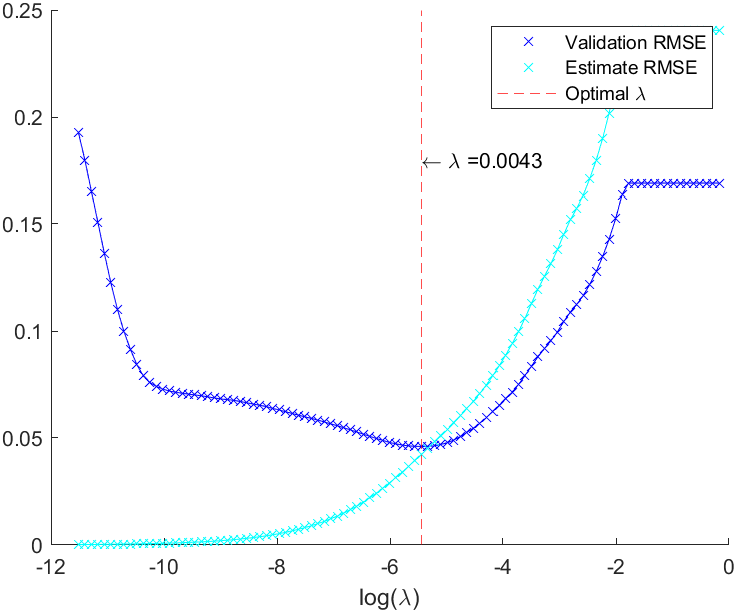
\includegraphics[width=0.7\textwidth]{task61.png}
    \caption{Validation and estimate RMSE for different $\lambda$.}
    \label{fig:my_label}
\end{figure}

As shown in figure 3, the regularization is needed in order to produce a clear reconstruction of the audio. No, or little regularization strength is shown to result in a noisy reconstruction as the validation RMSE is high for small $\lambda$. This also applies to strong regularization. However, there appears to be an optimum at $\lambda = 0.0043$.


\section{Task 7}
When listening to the original unfiltered audio, there was a significant amount of noise present. However, after filtering the noise using our model the sound was much more clear. Adjusting the $lambda$ for the model to a greater or lesser value both resulted in more distorted sound, indicating that optimal $\lambda$ proposed by the multiframe cross validation was very close to the actual optimal value.

\end{document}
